\chapter{Pembangunan Data Mart}

% ============================================================
%  7 PEMBANGUNAN DATA MART
% ============================================================
 
 
Data mart yang dibangun merupakan representasi fisik dari informasi yang telah dibersihkan, divalidasi, dan dioptimalkan, serta siap dikonsumsi secara langsung oleh jajaran manajemen rumah sakit untuk keperluan pengambilan keputusan strategis.
 
\section{Skema Final Data Mart}
 
Arsitektur fisik yang dipilih untuk Data Mart ini adalah \textbf{Skema Bintang (\textit{Star Schema}) Murni}. Skema bintang dipilih karena memiliki struktur yang sangat sederhana, mudah dipahami oleh pengguna bisnis, dan meminimalkan operasi penyambungan tabel (JOIN) yang kompleks. Hal ini membuat proses eksekusi \textit{query} agregasi pada \textit{Business Intelligence tools} menjadi sangat responsif.
 
Tabel Fakta (\texttt{fct\_kunjungan}) ditempatkan sebagai pusat dari arsitektur, mengumpulkan seluruh metrik kuantitatif transaksi medis. Tabel fakta ini kemudian dikelilingi dan diapit oleh lima Tabel Dimensi sebagai penjelas konteks peristiwa, yang terikat melalui hubungan \textit{One-to-Many} (1:N) dengan integritas referensial yang ketat.
 
\begin{center}
  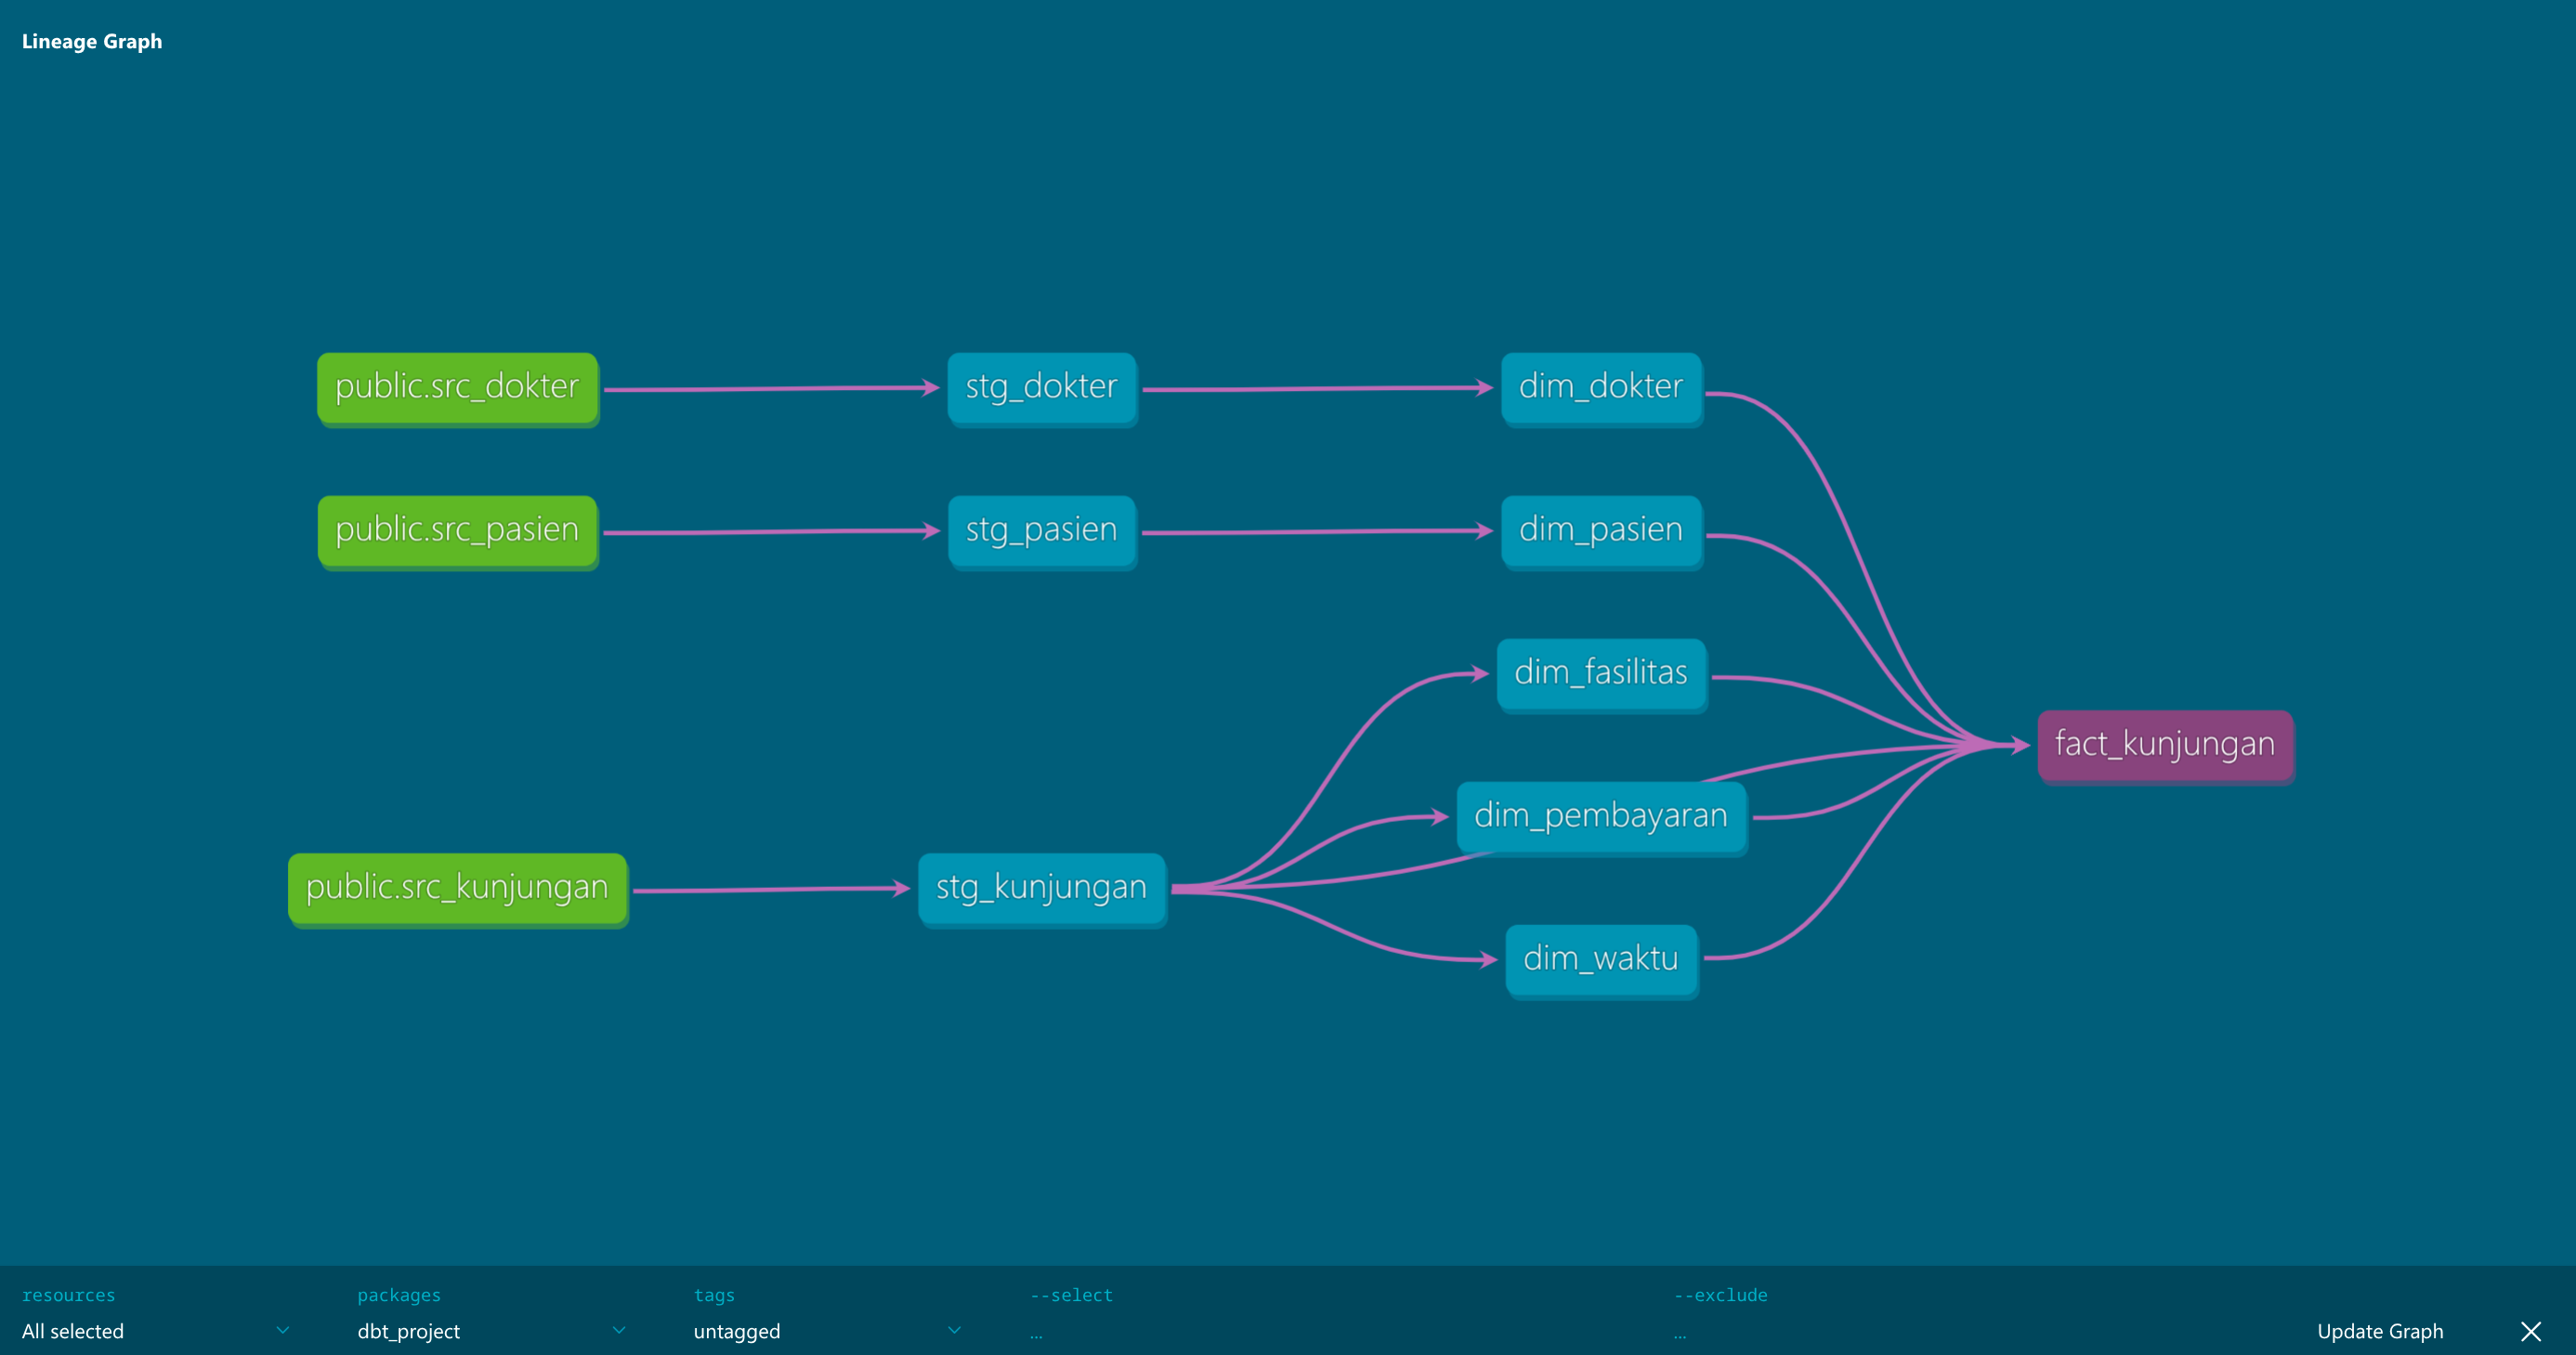
\includegraphics[width=0.95\textwidth]{./figures/5-4_DBT_lineage_graph.png}
  \captionof{figure}{Diagram ERD \textit{Star Schema} Final dari Database PostgreSQL.}
  \label{fig:5.4.erd_star_schema}
\end{center}
 
\section{Dokumentasi Tabel dan Kolom (Kamus Data)}
 
Guna memastikan kejelasan informasi dan menghindari ambiguitas data, berikut adalah spesifikasi teknis kamus data (\textit{data dictionary}) untuk tabel fakta dan tabel dimensi utama di dalam Data Mart.
 
\textbf{1. Tabel Fakta: \texttt{fct\_kunjungan}}
 
Deskripsi: Menyimpan rekam jejak transaksi kunjungan pasien, durasi pelayanan, serta rincian biaya finansial yang terjadi di rumah sakit. Materialisasi: \texttt{Table} (Fisik).
 
\begin{table}[H]
\centering
\caption{Kamus Data Tabel Fakta \texttt{fct\_kunjungan}}
\small
\begin{tabularx}{\linewidth}{p{3cm}p{2.2cm}p{2.4cm}p{3cm}X}
\toprule
\textbf{Nama Kolom} & \textbf{Tipe Data} & \textbf{Peran} & \textbf{Aturan Validasi} & \textbf{Deskripsi Fungsional} \\
\midrule
\texttt{kunjungan\_key}   & VARCHAR(50)   & Primary Key (PK)   & unique, not\_null                           & Kode hash unik per transaksi kunjungan. \\
\texttt{pasien\_key}      & INT           & Foreign Key (FK)   & not\_null, rel.\ ke \texttt{dim\_pasien}    & Kunci relasi ke master data pasien. \\
\texttt{dokter\_key}      & INT           & Foreign Key (FK)   & not\_null, rel.\ ke \texttt{dim\_dokter}    & Kunci relasi ke master data dokter pemeriksa. \\
\texttt{waktu\_key}       & INT           & Foreign Key (FK)   & not\_null, rel.\ ke \texttt{dim\_waktu}     & Kunci relasi ke kalender dimensi temporal. \\
\texttt{fasilitas\_key}   & VARCHAR(50)   & Foreign Key (FK)   & not\_null                                   & Kunci relasi ke klaster jenis fasilitas. \\
\texttt{pembayaran\_key}  & VARCHAR(50)   & Foreign Key (FK)   & not\_null                                   & Kunci relasi ke dimensi metode pembayaran. \\
\texttt{durasi\_rawat}    & INT           & Measure            & nilai $\geq 0$                              & Lama waktu pasien dirawat (satuan: hari). \\
\texttt{biaya\_konsultasi}& NUMERIC(15,2) & Measure            & nilai $\geq 0$                              & Nominal biaya untuk jasa pemeriksaan dokter. \\
\texttt{biaya\_obat}      & NUMERIC(15,2) & Measure            & nilai $\geq 0$                              & Nominal biaya pengadaan obat-obatan pasien. \\
\texttt{biaya\_tindakan}  & NUMERIC(15,2) & Measure            & nilai $\geq 0$                              & Nominal biaya pengerjaan prosedur medis/operasi. \\
\texttt{biaya\_kamar}     & NUMERIC(15,2) & Measure            & nilai $\geq 0$                              & Nominal biaya sewa ruang rawat inap. \\
\texttt{total\_biaya}     & NUMERIC(15,2) & Calculated Measure & nilai $\geq 0$                              & Akumulasi total biaya keseluruhan layanan medis. \\
\bottomrule
\end{tabularx}
\end{table}
 
\textbf{2. Tabel Dimensi: \texttt{dim\_pasien}}
 
Deskripsi: Menyimpan profil demografis master seluruh pasien rumah sakit. Materialisasi: \texttt{Table} (Fisik).
 
\begin{table}[H]
\centering
\caption{Kamus Data Tabel Dimensi \texttt{dim\_pasien}}
\small
\begin{tabularx}{\linewidth}{p{2.8cm}p{2cm}p{2.8cm}p{2.8cm}X}
\toprule
\textbf{Nama Kolom} & \textbf{Tipe Data} & \textbf{Peran} & \textbf{Aturan Validasi} & \textbf{Deskripsi Fungsional} \\
\midrule
\texttt{pasien\_key}    & INT          & Primary Key (PK)   & unique, not\_null                          & \textit{Surrogate Key} numerik untuk entitas pasien. \\
\texttt{pasien\_id}     & VARCHAR(30)  & Natural Key        & not\_null                                  & Nomor rekam medis asli dari sistem operasional. \\
\texttt{nama\_pasien}   & VARCHAR(150) & Atribut Deskriptif & not\_null                                  & Nama lengkap pasien sesuai kartu identitas. \\
\texttt{jenis\_kelamin} & VARCHAR(15)  & Atribut Deskriptif & nilai \texttt{'L'} atau \texttt{'P'}        & Jenis kelamin pasien untuk analisis demografi. \\
\texttt{tanggal\_lahir} & DATE         & Atribut Deskriptif & not\_null                                  & Tanggal lahir untuk kalkulasi kelompok usia. \\
\texttt{alamat}         & TEXT         & Atribut Deskriptif & --                                         & Wilayah tempat tinggal pasien saat ini. \\
\bottomrule
\end{tabularx}
\end{table}
 
\textbf{3. Tabel Dimensi: \texttt{dim\_dokter}}
 
Deskripsi: Menyimpan informasi profil dokter dan spesialisasi medis yang tersedia di rumah sakit. Materialisasi: \texttt{Table} (Fisik).
 
\begin{table}[H]
\centering
\caption{Kamus Data Tabel Dimensi \texttt{dim\_dokter}}
\small
\begin{tabularx}{\linewidth}{p{2.8cm}p{2cm}p{2.8cm}p{2.8cm}X}
\toprule
\textbf{Nama Kolom} & \textbf{Tipe Data} & \textbf{Peran} & \textbf{Aturan Validasi} & \textbf{Deskripsi Fungsional} \\
\midrule
\texttt{dokter\_key}   & INT          & Primary Key (PK)   & unique, not\_null & \textit{Surrogate Key} numerik untuk entitas dokter. \\
\texttt{dokter\_id}    & VARCHAR(30)  & Natural Key        & not\_null         & ID unik dokter dari sistem operasional kepegawaian. \\
\texttt{nama\_dokter}  & VARCHAR(150) & Atribut Deskriptif & not\_null         & Nama lengkap dokter beserta gelar medisnya. \\
\texttt{spesialisasi}  & VARCHAR(100) & Atribut Deskriptif & not\_null         & Bidang keahlian spesialisasi dokter (misal: Anak, Dalam). \\
\bottomrule
\end{tabularx}
\end{table}
 
\section{Koneksi ke Business Intelligence (BI) Tools}
 
Data Mart ini menetap secara permanen di dalam database PostgreSQL pada skema \texttt{public}. Berdasarkan konfigurasi file \texttt{docker-compose.yaml} yang telah dimodifikasi, \textit{port} internal container database telah dibuka dan dipetakan menuju jaringan luar \textit{host} lokal melalui instruksi ekspos \textit{port} (\texttt{ports: - "5432:5432"}).
 
Proses integrasi antara lapisan Data Mart (PostgreSQL) dengan \textit{Business Intelligence Tool} (Metabase) dilakukan melalui serangkaian tahapan inisialisasi parameter lingkungan (\textit{onboarding wizard}) hingga konfigurasi jaringan relasional. Berdasarkan arsitektur Docker yang didefinisikan pada berkas \texttt{docker-compose.yaml}, layanan database PostgreSQL berjalan secara internal pada \textit{port} 5432, namun diekspos ke jaringan \textit{host} lokal melalui pemetaan \textit{port} eksternal \texttt{5555:5432}. Oleh karena itu, pengaturan rute komunikasi pada Metabase harus disesuaikan secara presisi agar data hasil transformasi dbt dapat dibaca dengan sempurna.
 
Berikut adalah langkah-langkah sistematis konfigurasi koneksi dari awal hingga berhasil:
 
\begin{enumerate}
 
  \item \textbf{Inisialisasi dan Pemilihan Bahasa Utama}
  \begin{center}
    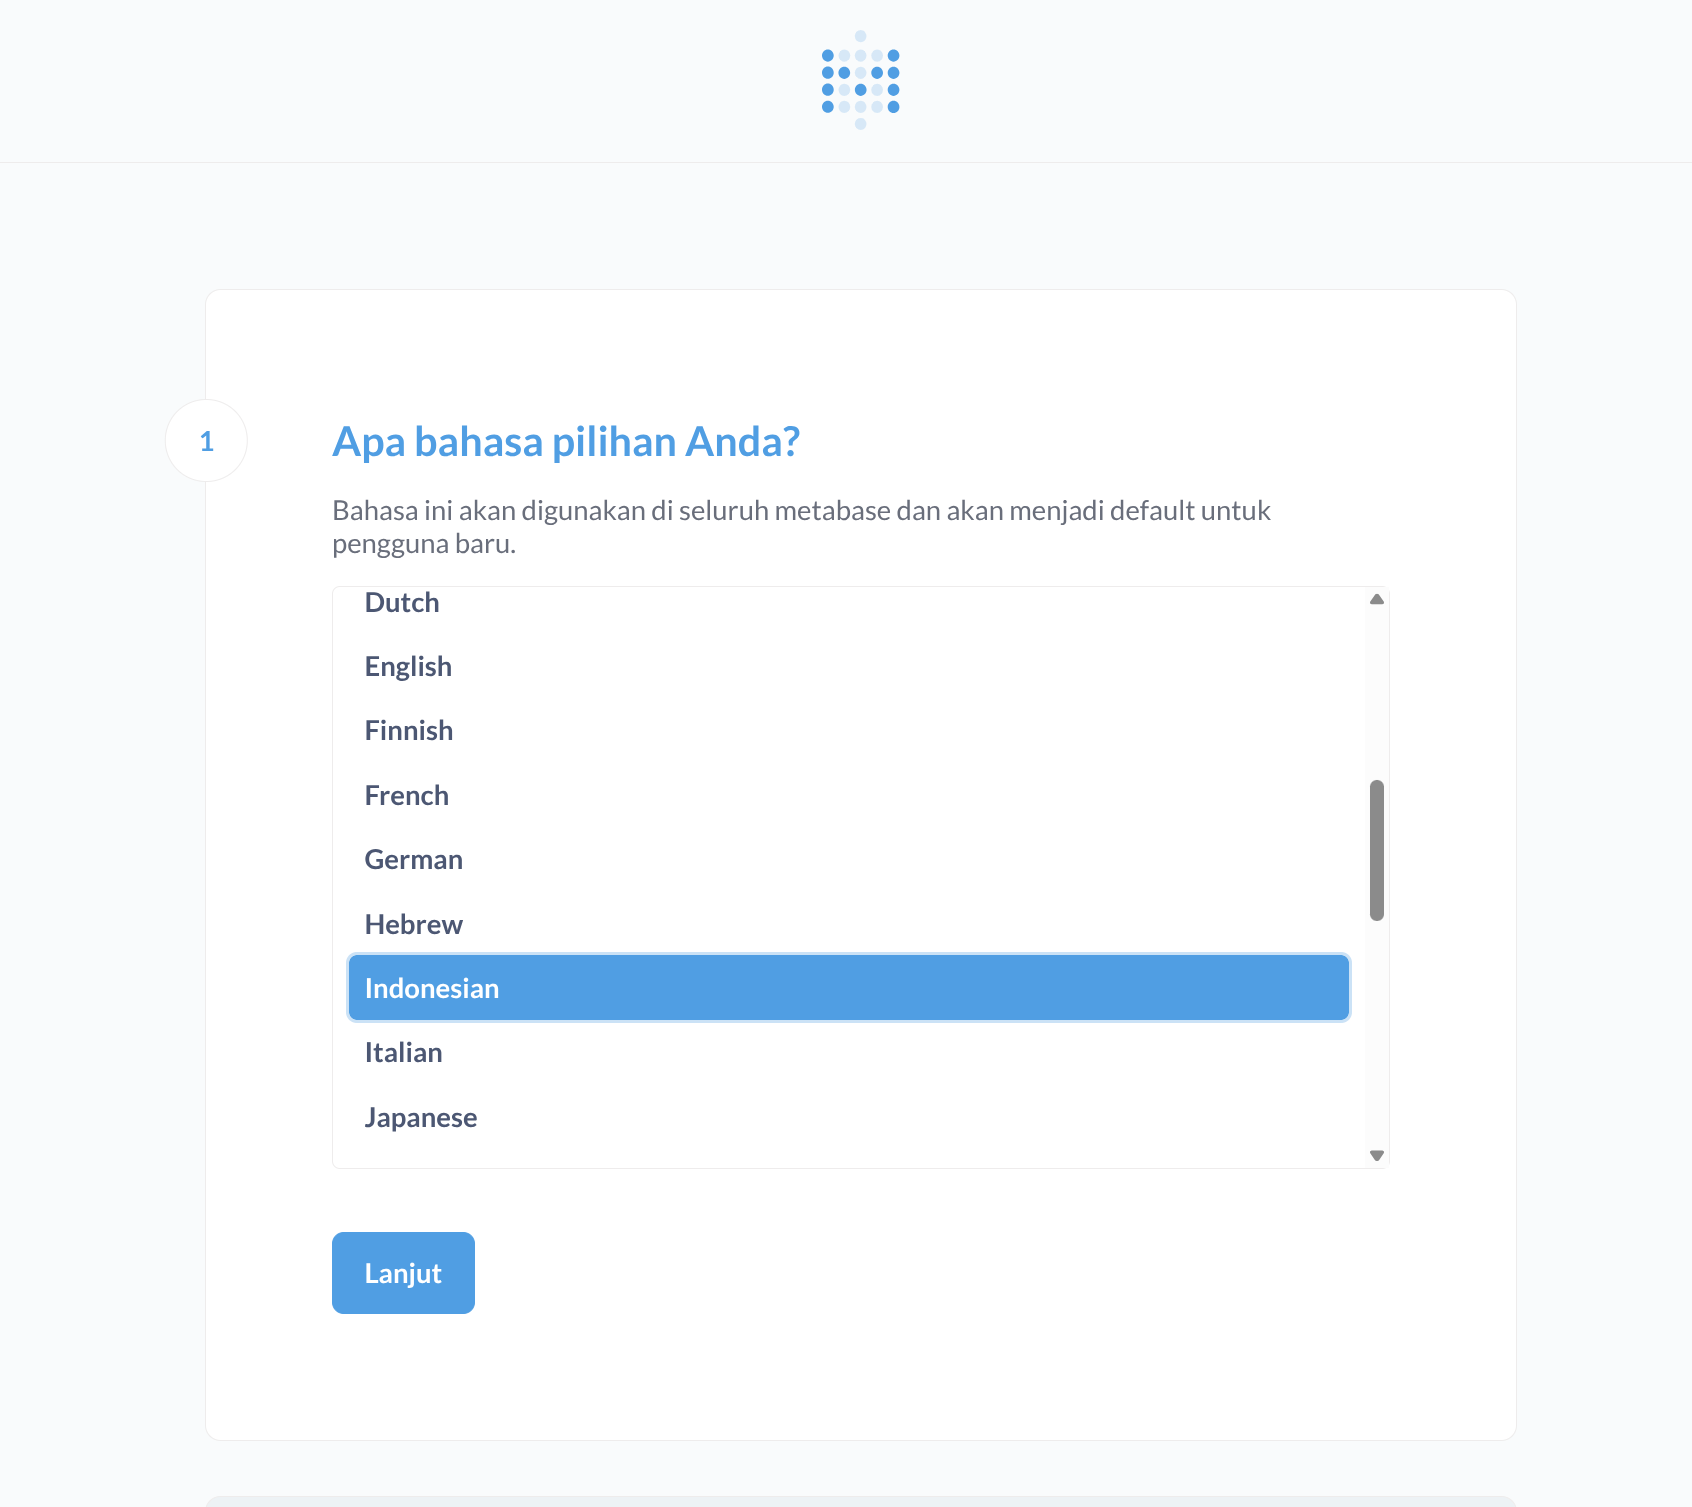
\includegraphics[width=0.75\textwidth]{./figures/5-5_mbase_01.png}
    \captionof{figure}{Halaman pemilihan bahasa pada inisialisasi awal Metabase.}
    \label{fig:5-5_mbase_01.png}
  \end{center}
  
  Saat pertama kali mengakses antarmuka Metabase via peramban web, pengguna disambut oleh menu preferensi bahasa lokalisasi. Pada tahapan ini, dipilih bahasa \textit{Indonesian (Indonesia)} sebagai bahasa bawaan sistem (\textit{default language}) untuk mempermudah navigasi seluruh pengguna dan jajaran manajemen di dalam ekosistem analitik rumah sakit ini.
 
 
  \item \textbf{Pembuatan Akun Administrator Perangkat}
   \begin{center}
    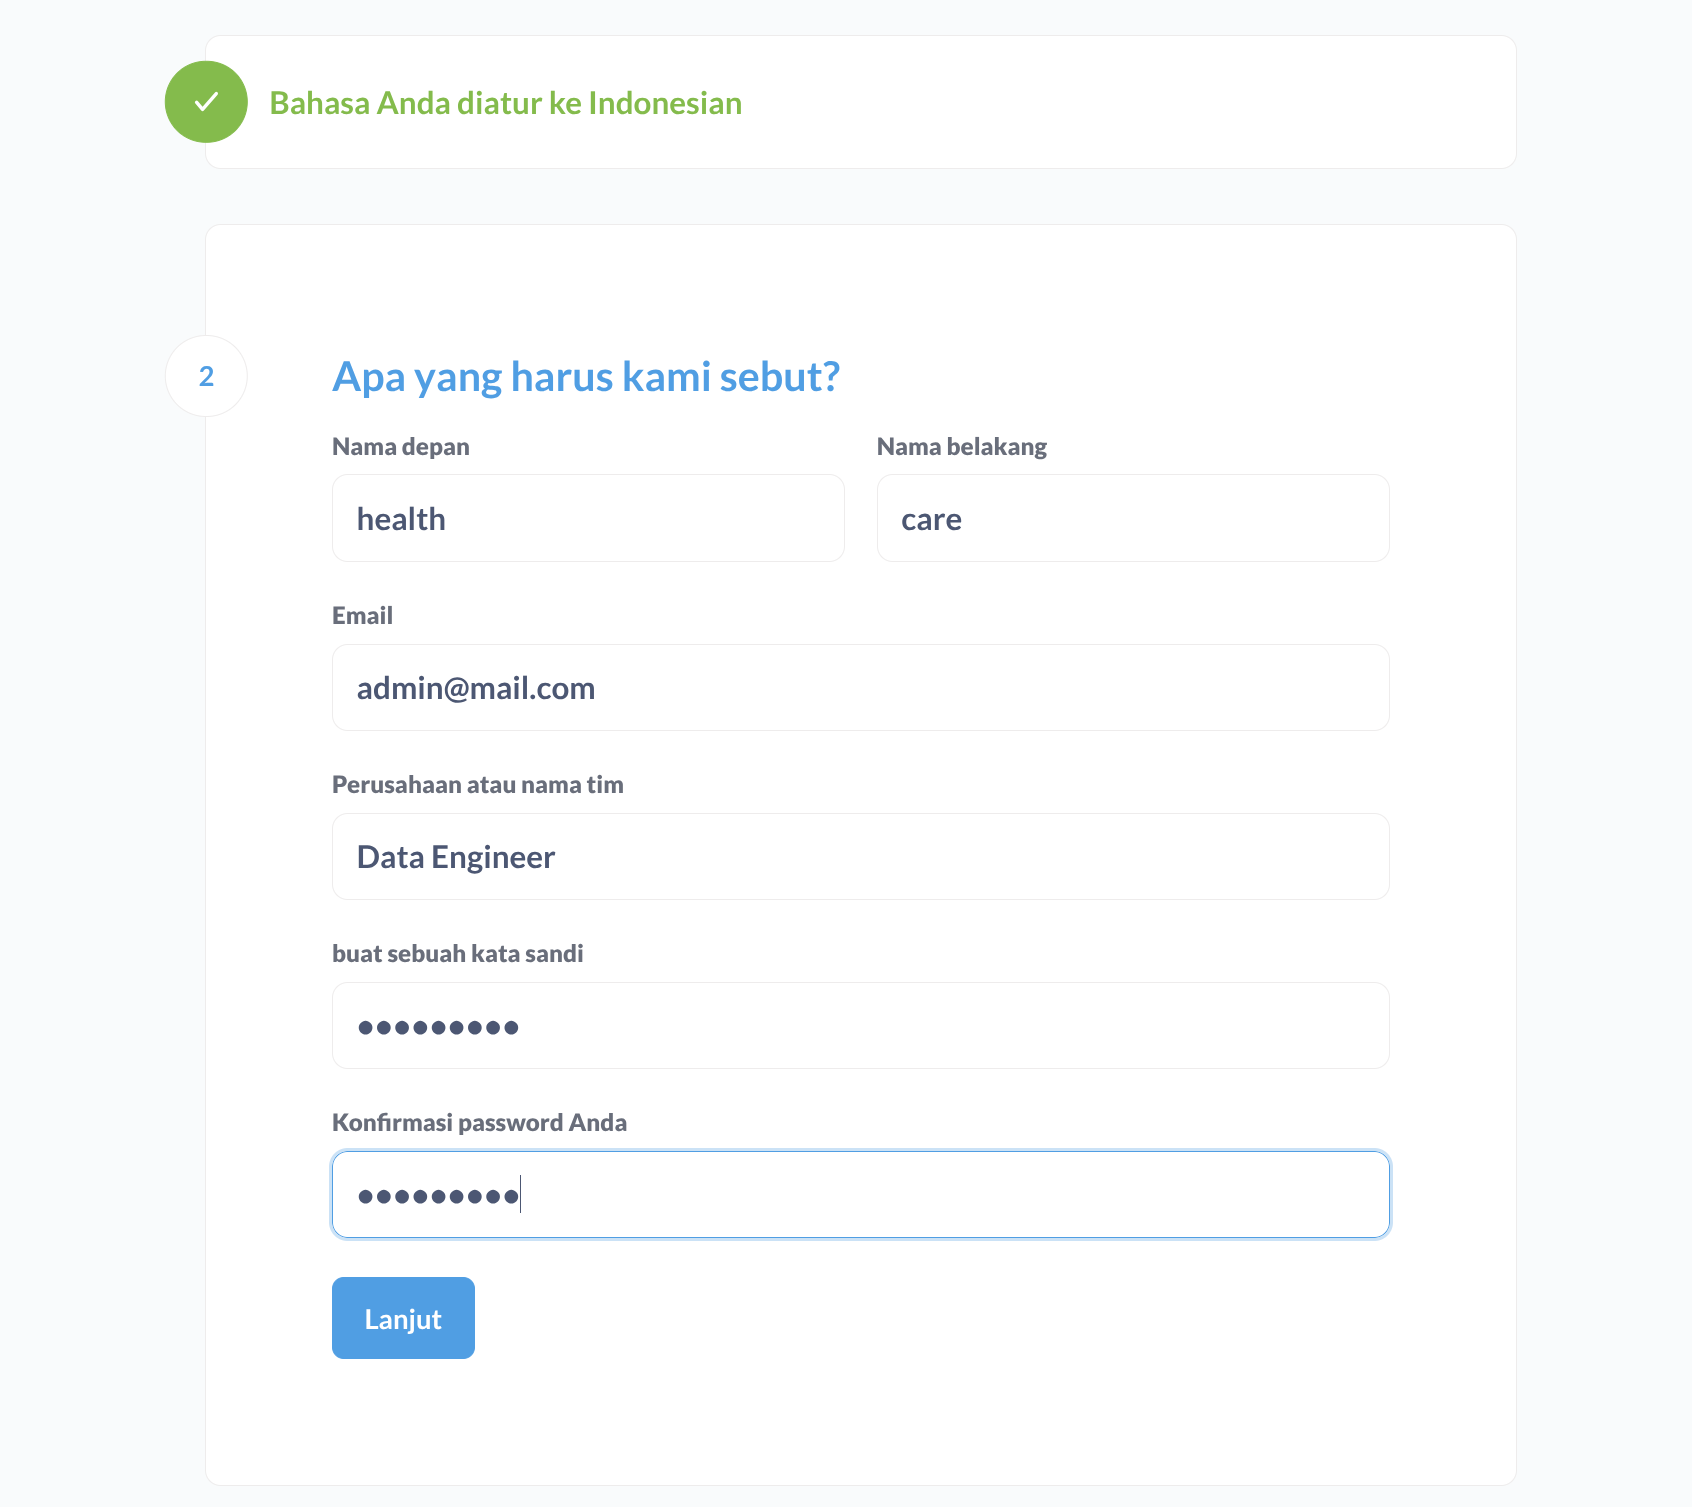
\includegraphics[width=0.75\textwidth]{./figures/5-5_mbase_02.png}
    \captionof{figure}{Halaman pembuatan akun administrator pada inisialisasi Metabase.}
    \label{fig:5-5_mbase_02.png}
  \end{center}

  Langkah kedua adalah mengamankan sistem dengan membangun kredensial pengguna utama (\textit{Superadmin/Administrator}). Akun ini memegang hak akses penuh terhadap manajemen database, pembuatan dasbor, serta pembagian hak akses pengguna operasional. Parameter yang didaftarkan adalah sebagai berikut:
 
  \begin{itemize}
    \item Nama Depan \& Belakang: \texttt{health care}
    \item Alamat Email: \texttt{admin@mail.com}
    \item Perusahaan / Nama Tim: \texttt{Data Engineer}
    \item Kata Sandi: (diatur secara aman untuk pemenuhan jaminan keamanan data pasien)
  \end{itemize}
 
  \item \textbf{Penentuan Orientasi Penggunaan Perangkat (Survey)}
   \begin{center}
    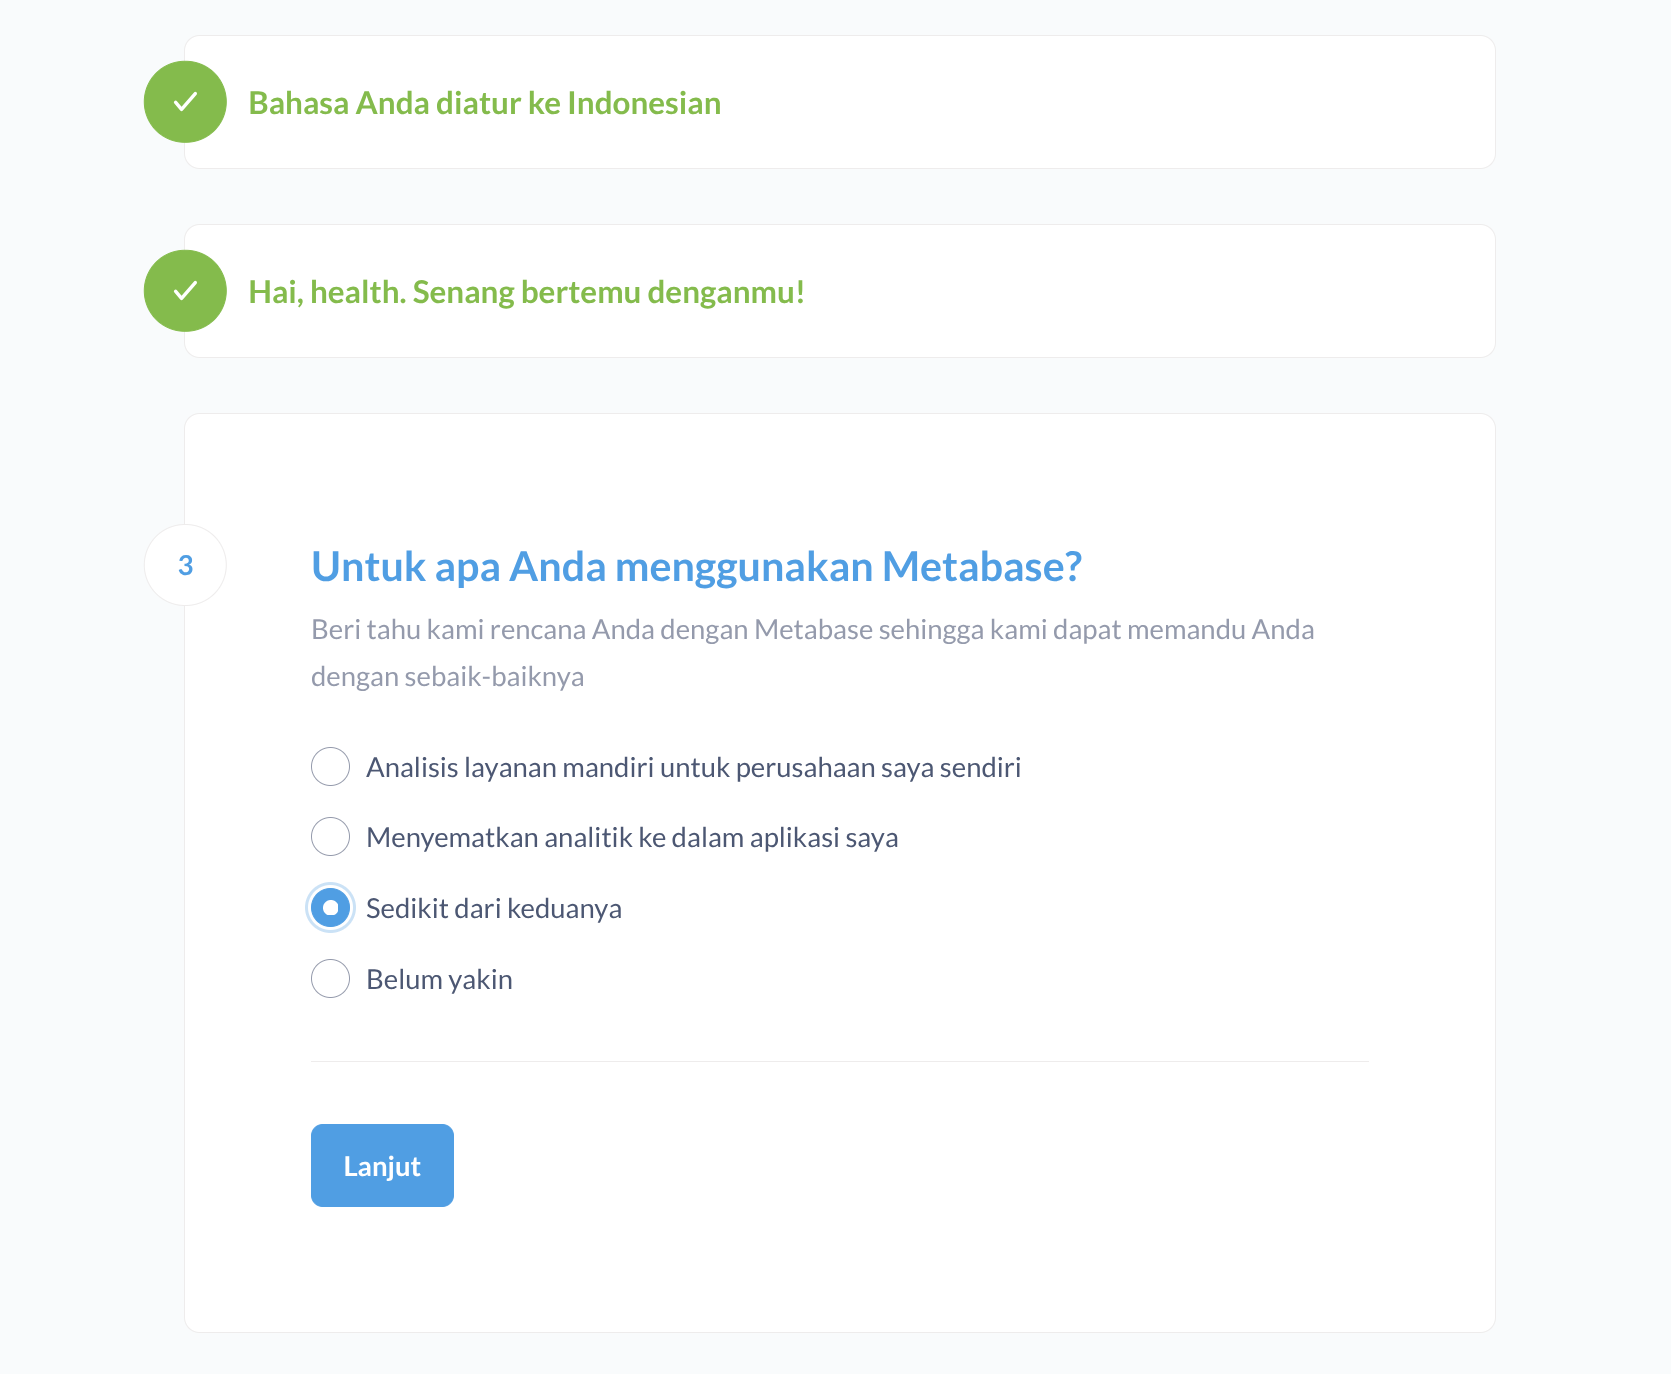
\includegraphics[width=0.75\textwidth]{./figures/5-5_mbase_03.png}
    \captionof{figure}{Halaman survey orientasi penggunaan pada inisialisasi Metabase.}
    \label{fig:5-5_mbase_03.png}
  \end{center}

  Metabase menyajikan kuesioner singkat untuk mengoptimalkan mesin visualisasi sesuai kebutuhan organisasi. Pilihan jatuh pada opsi \textit{"Sedikit dari keduanya"}, yang menandakan bahwa Metabase akan difungsikan secara hibrida: baik untuk kebutuhan analisis data mandiri (\textit{self-service analytics} oleh tim manajemen medis) maupun untuk penyematan grafik analitik ke dalam aplikasi operasional rumah sakit yang lebih luas.
 
  \item \textbf{Pemilihan Jenis Database (DBMS Target)}
  \begin{center}
    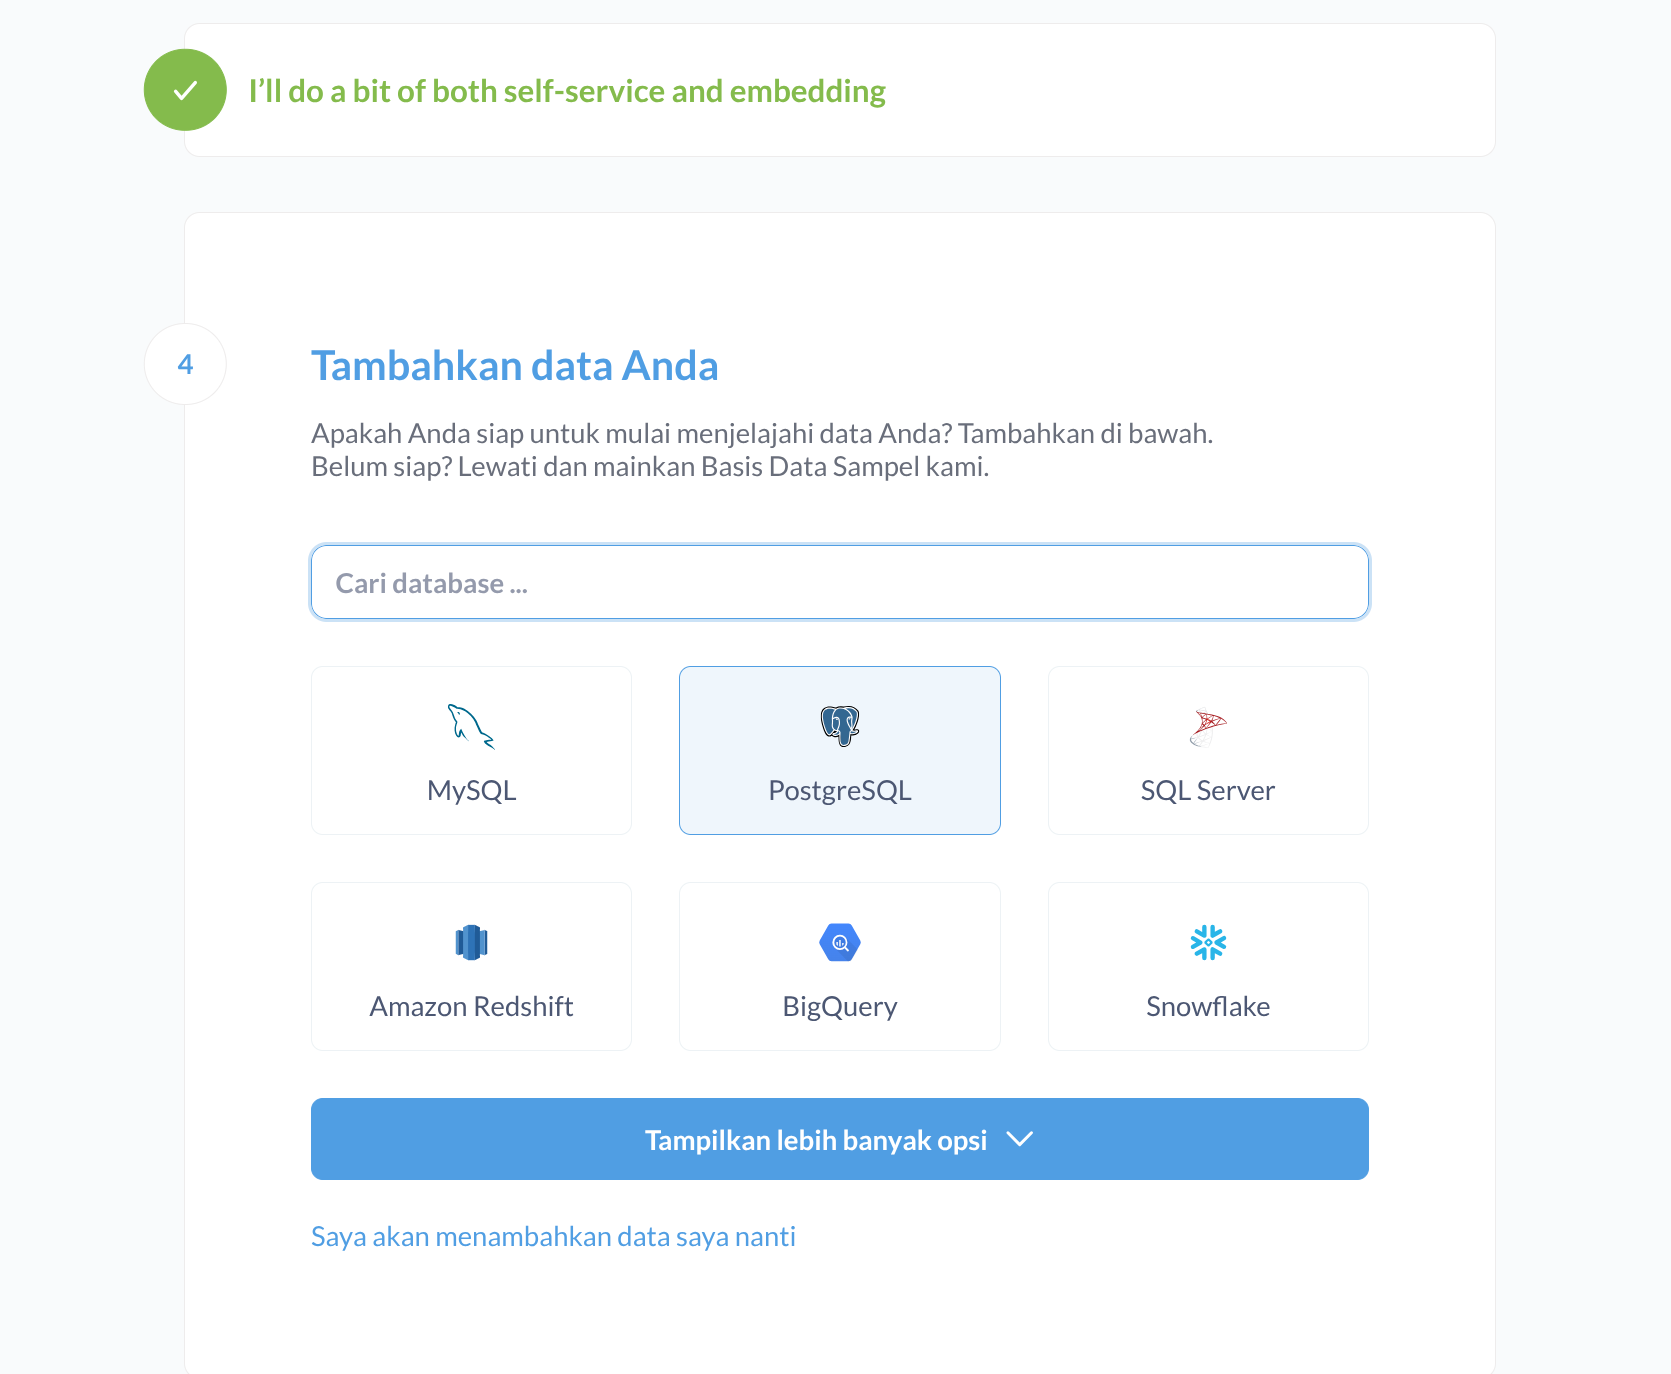
\includegraphics[width=0.75\textwidth]{./figures/5-5_mbase_04.png}
    \captionof{figure}{Halaman pemilihan tipe database pada inisialisasi Metabase.}
    \label{fig:5-5_mbase_04.png}
  \end{center}

  Metabase mendukung konektivitas ke puluhan sistem database modern. Karena Data Mart proyek ini dibangun di atas infrastruktur PostgreSQL (sesuai konfigurasi \texttt{postgres:13} di Docker), maka ikon PostgreSQL dipilih sebagai tipe database tujuan utama untuk membuka \textit{form} pemetaan skema relasional.
 
  \item \textbf{Analisis Percobaan Pertama Koneksi Jaringan (Uji Coba Port 5432)}
  \begin{center}
    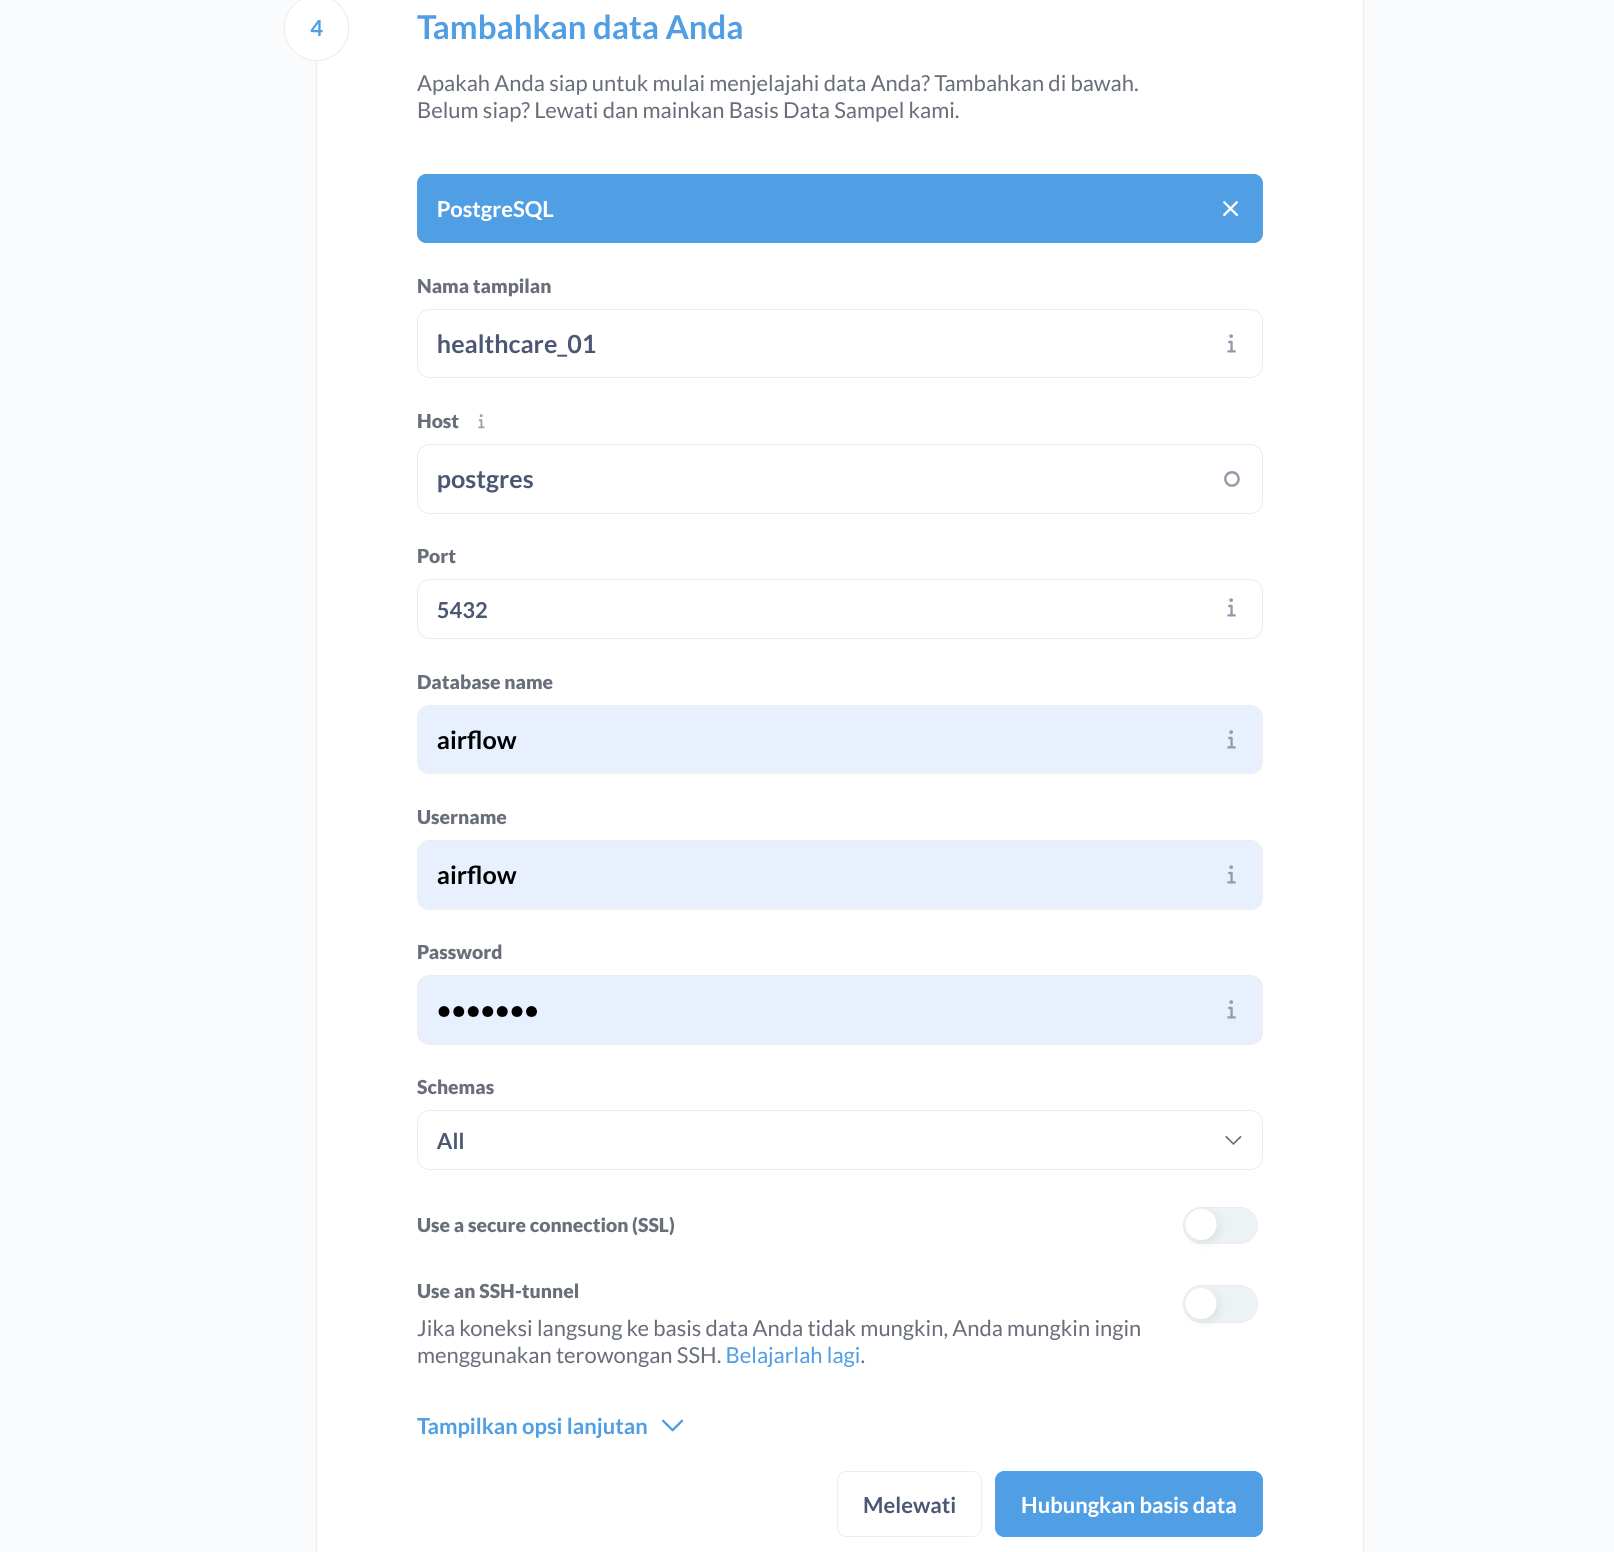
\includegraphics[width=0.75\textwidth]{./figures/5-5_mbase_05.png}
    \captionof{figure}{Parameter database PostgreSQL pada wizard Metabase.}
    \label{fig:5-5_mbase_05.png}
  \end{center}
 
  Pada pengisian \textit{form} awal, dilakukan uji coba pengisian parameter penghubung menggunakan \textit{port} standar PostgreSQL internal dengan komponen data sebagai berikut:
 
  \begin{table}[H]
  \centering
  \small
  \begin{tabularx}{0.75\linewidth}{lX}
  \toprule
  \textbf{Parameter} & \textbf{Nilai} \\
  \midrule
  Nama Tampilan & \texttt{healthcare} \\
  Host          & \texttt{host.docker.internal} \\
  Port          & \texttt{5432} \\
  Database Name & \texttt{airflow} \\
  Username      & \texttt{airflow} \\
  Password      & \texttt{airflow} \\
  \bottomrule
  \end{tabularx}
  \end{table}
 
  \begin{mybox}{Analisis Teknis: Batasan Port 5432}
  Konfigurasi \textit{port} 5432 pada tahap ini hanya akan berhasil jika Metabase dijalankan di dalam klaster jaringan internal Docker yang sama (\textit{same network bridge}). Jika Metabase bertindak dari luar jaringan Docker, \textit{port} ini akan ditolak oleh sistem karena adanya restriksi isolasi kontainer.
  \end{mybox}
 
  \item \textbf{Pengaturan Preferensi Pelacakan Data Anonim}
  \begin{center}
    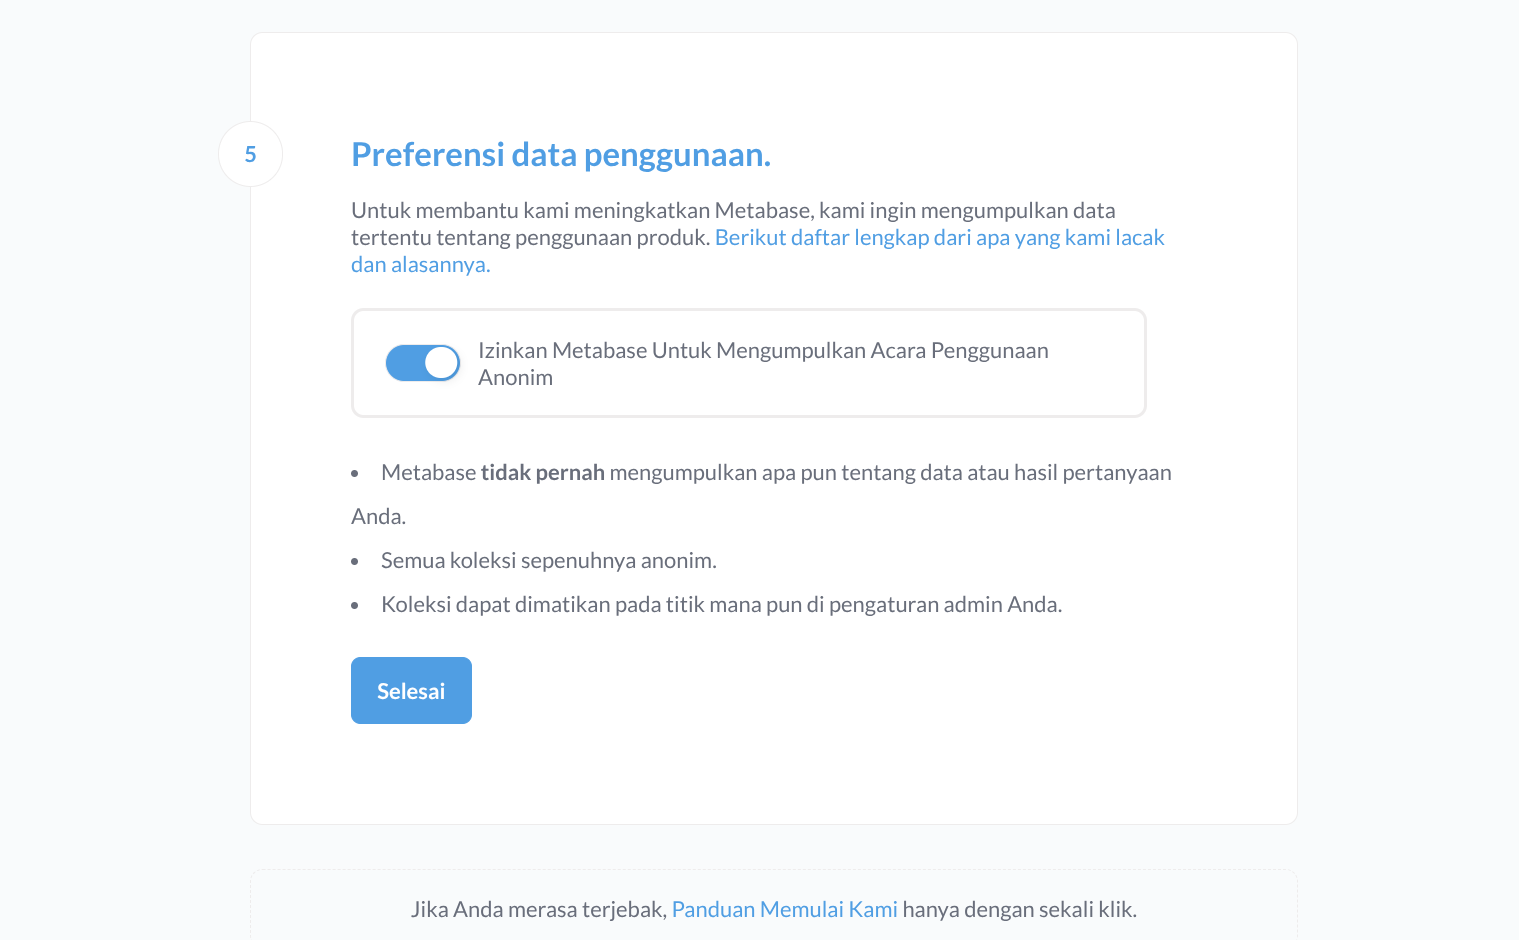
\includegraphics[width=0.75\textwidth]{./figures/5-5_mbase_06.png}
    \captionof{figure}{Pengaturan Preferensi Pelacakan Data Anonim pada wizard Metabase.}
    \label{fig:5-5_mbase_06.png}
  \end{center}

  Sebelum proses instalasi selesai, sistem meminta persetujuan terkait pelacakan data penggunaan performa aplikasi. Opsi \textit{"Izinkan Metabase Untuk Mengumpulkan Acara Penggunaan Anonim"} diaktifkan guna membantu komunitas pengembang Metabase menerima laporan telemetri \textit{bug} secara otomatis tanpa melanggar privasi data rekam medis pasien, karena data \textit{query} tabel tetap bersifat rahasia dan terisolasi lokal.
 
  \item \textbf{Penyelesaian Onboarding Awal Perangkat}
  \begin{center}
    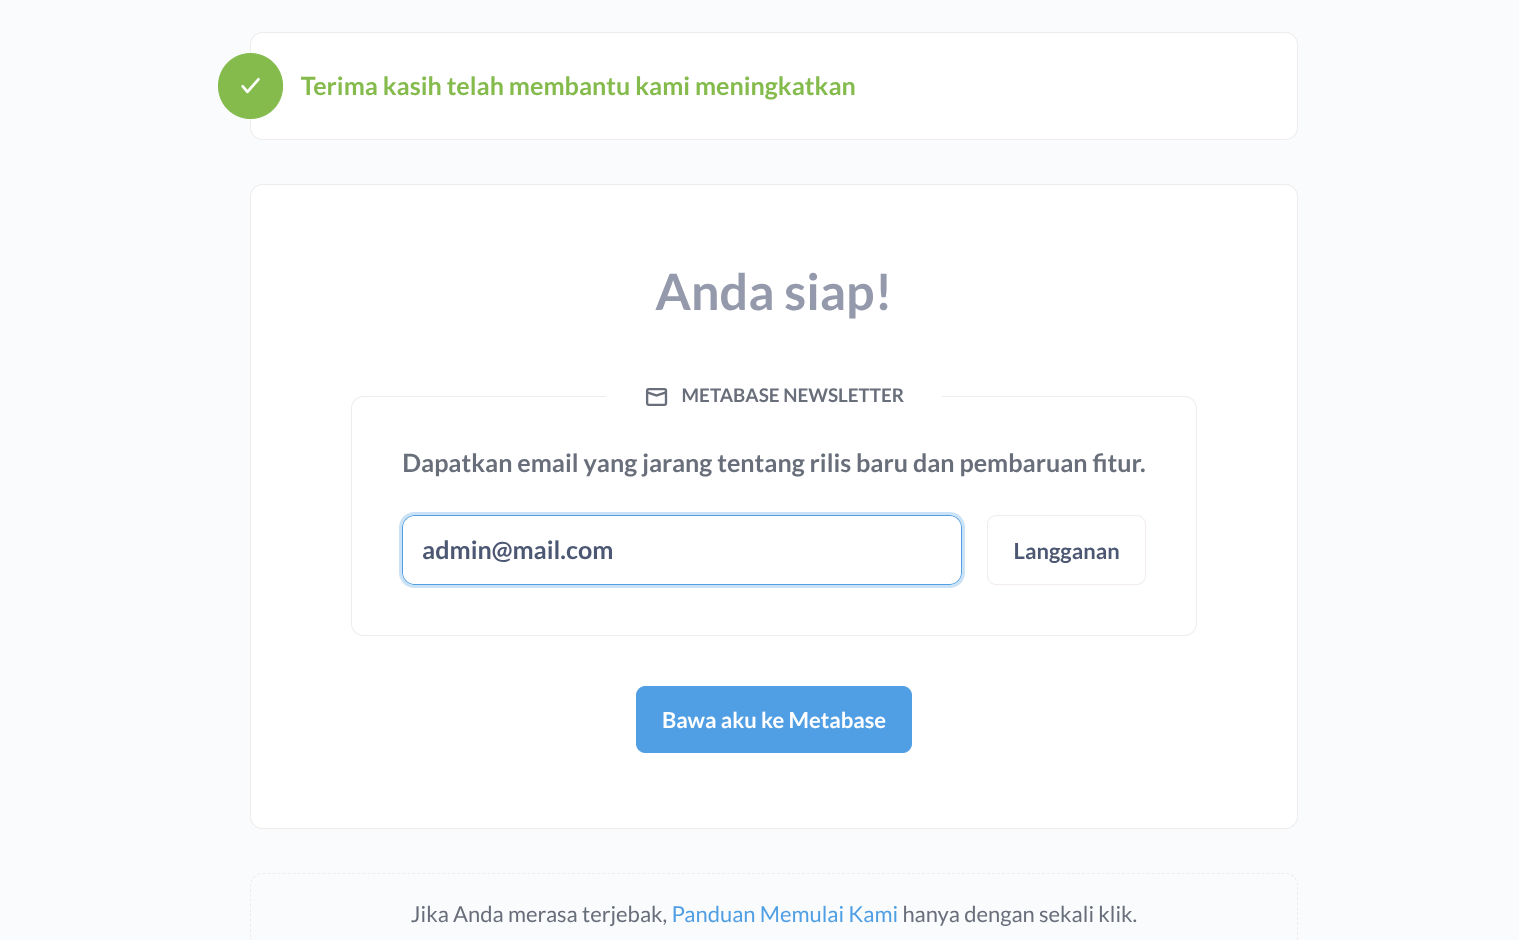
\includegraphics[width=0.75\textwidth]{./figures/5-5_mbase_07.png}
    \captionof{figure}{Penyelesaian Onboarding Awal Perangkat pada wizard Metabase.}
    \label{fig:5-5_mbase_07.png}
  \end{center}
 
  Tahapan \textit{onboarding wizard} dinyatakan berhasil ditandai dengan munculnya pesan konfirmasi \textit{"Anda siap!"}. Di halaman ini, email administrator (\texttt{admin@mail.com}) dimasukkan kembali ke dalam \textit{form} buletin informasi untuk berlangganan pembaruan fitur keamanan penting dari Metabase.
  
  \item \textbf{Akses Masuk ke Panel Administrasi Utama (\textit{Admin Settings})}
  \begin{center}
    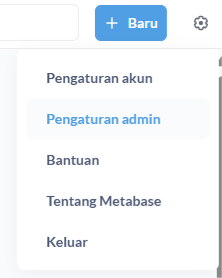
\includegraphics[width=0.75\textwidth]{./figures/5-5_mbase_08.png}
    \captionof{figure}{Akses ke Panel Administrasi Utama pada wizard Metabase.}
    \label{fig:5-5_mbase_08.png}
  \end{center}

  Setelah masuk ke halaman beranda utama Metabase, pengguna diarahkan menuju pojok kanan atas untuk membuka ikon gerigi pengaturan (\textit{Settings}) dan masuk ke submenu \textit{"Pengaturan admin"}. Langkah ini krusial untuk melakukan perbaikan dan validasi ulang koneksi database yang sempat tertunda atau mengalami kendala rute \textit{port} eksternal.
 
  \item \textbf{Konfigurasi Sukses Koneksi Final Data Mart (Penerapan Port Forwarding 5555)}
  \begin{center}
    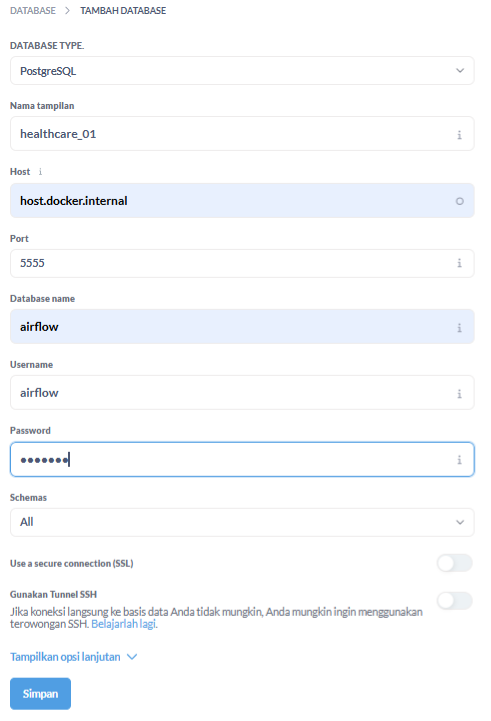
\includegraphics[width=0.75\textwidth]{./figures/5-5_mbase_09.png}
    \captionof{figure}{Konfigurasi Koneksi Final Data Mart pada wizard Metabase.}
    \label{fig:5-5_mbase_09.png}
  \end{center}

  Pada panel administrasi, di bawah menu \textit{"Tambah Database"}, dilakukan perbaikan parameter koneksi agar selaras dengan deklarasi pemetaan \textit{port} luar pada file \texttt{docker-compose.yaml} (\texttt{ports: - "5555:5432"}). Spesifikasi parameter final yang dimasukkan adalah sebagai berikut:
 
  \begin{table}[H]
  \centering
  \caption{Parameter Koneksi Final Data Mart ke Metabase}
  \begin{tabularx}{0.85\linewidth}{lX}
  \toprule
  \textbf{Parameter} & \textbf{Nilai} \\
  \midrule
  Database Type  & PostgreSQL \\
  Nama Tampilan  & \texttt{healthcare\_01} \\
  Host           & \texttt{host.docker.internal} \\
  Port           & \texttt{5555} \\
  Database Name  & \texttt{airflow} \\
  Username       & \texttt{airflow} \\
  Password       & \texttt{airflow} \\
  Schemas        & All \\
  \bottomrule
  \end{tabularx}
  \end{table}

 
  \begin{mybox}{Catatan: Port Forwarding 5555}
  \textit{Port} wajib diubah menjadi \texttt{5555} karena Metabase mengakses PostgreSQL dari sisi \textit{host} eksternal, memanfaatkan pintu gerbang \textit{forwarding} yang telah disediakan Docker. Setelah tombol \textit{"Simpan"} ditekan, Metabase akan melakukan \textit{handshake protocol} ke database PostgreSQL. Status keberhasilan ditandai dengan hilangnya pesan \textit{error} dan dimulainya proses sinkronisasi skema metadata secara otomatis (\textit{scanning tables}).
  \end{mybox}
 
\end{enumerate}
 
Dengan tuntasnya langkah ke-9, Data Mart kesehatan kini telah terhubung secara sempurna dengan Metabase. Proses \textit{query} interaktif, pembuatan visualisasi grafik kunjungan, analisis biaya medis, serta pembuatan dasbor eksekutif siap dilakukan pada tahapan berikutnya. BI Tools seperti Metabase, Apache Superset, Tableau, atau Power BI dapat langsung membaca seluruh daftar tabel \texttt{dim\_*} dan \texttt{fct\_kunjungan} untuk mulai menyusun grafik, diagram, serta dasbor pemantauan kinerja rumah sakit.
 
\section{Lapisan Semantik (\textit{Semantic Layer})}
 
Untuk menjamin konsistensi metrik bisnis dan menghindari kesalahan penafsiran rumus oleh tim analis yang berbeda, proyek ini menerapkan konsep \textbf{\textit{Semantic Layer}} (Lapisan Semantik). Logika kalkulasi bisnis dipusatkan dan dikunci di tingkat dbt, sehingga BI Tools hanya perlu memanggil metrik yang sudah matang tanpa perlu menulis ulang fungsi agregasi yang rumit.
 
Metrik utama yang didefinisikan secara baku pada lapisan semantik ini meliputi:
 
\begin{itemize}
  \item \textbf{Metrik Finansial (Total Pendapatan Rumah Sakit):} Ditentukan secara mutlak melalui formula penjumlahan komponen biaya operasional pada tabel fakta kunjungan:
  \[
    \text{Total Biaya} = \text{Biaya Konsultasi} + \text{Biaya Obat}
      + \text{Biaya Tindakan} + \text{Biaya Kamar}
  \]
 
  \item \textbf{Metrik Efisiensi Operasional (\textit{Average Length of Stay} / Avg LoS):} Digunakan untuk mengukur efektivitas utilitas tempat tidur perawatan, dirumuskan melalui fungsi agregasi rata-rata:
  \[
    \text{Avg LoS} = \text{AVG}(\texttt{durasi\_rawat})
  \]
 
  \item \textbf{Metrik Kuantitas (Total Kunjungan Medis):} Dirumuskan melalui fungsi perhitungan unik terhadap kunci utama kunjungan:
  \[
    \text{Total Kunjungan} = \text{COUNT}(\texttt{kunjungan\_key})
  \]
\end{itemize}
 
\begin{mybox}{Catatan: Single Source of Truth}
Dengan diterapkannya \textit{Semantic Layer} ini, seluruh laporan visual yang diproduksi oleh BI tools yang berbeda dijamin akan menyajikan angka KPI yang seragam, konsisten, valid, dan menjadi satu-satunya acuan kebenaran data (\textit{Single Source of Truth}) bagi organisasi rumah sakit.
\end{mybox}